\section{Methoden} \label{sec:Methoden}
			
	Zum Versuchsaufbau gehören ein Elektromagnet, eine Stromquelle, eine Hall-Sonde, zwei Polarisatoren, ein (roter) Laser, einer Photodiode und eine Co/Pt-Probe.
	Der Elektromagnet besteht aus einem hufeisenförmigen Eisenkern, auf dessen Seiten Spulen mit je 600 Windungen angebracht sind, durch die ein Strom aus der Stromquelle fließen kann. 
	Zudem sind an den Enden des Eisenkerns Polschuhe angebracht, zwischen denen sich ein Magnetfeld bei Stromfluss durch die Spulen bilden sollte.
	Für den ersten Versuchsteil soll die Feldstärke $B$ dieses Magnetfeldes in Abhängigkeit der Stromstärke $I$ über die Hall-Sonde gemessen werden.
	Dazu wird die Sonde so ausgerichtet, dass möglichst parallel zu dem Magnetfeld gemessen werden kann.
	Bei dem zweiten Versuchsteil soll die Hall-Sonde entfernt und die Co/Pt-Probe zwischen den Polschuhen platziert werden.
	Der Laser wird so aufgestellt, dass ein gerader Strahlengang durch den ersten Polarisator auf die Probe und des reflektierten Strahls durch den zweiten Polarisator stattfinden kann.
	Hinter letzterem soll dann die Lichtintensität $U$ in Abhängigkeit der Stromstärke $I$ (der magnetischen Feldstärke $B$) mit der Photodiode gemessen werden.
	Für höhere Empfindlichkeit sollen die Polarisatoren um \SI{45}{\degree} versetzt polarisieren, da die Änderung der Intensität nach dem Gesetz von Malus dann am größten ist.
	Bei beiden Messungen sollen die Messgrößen in Abhängigkeit Stromstärke von \SIrange{-1}{1}{\ampere}	und wieder zurück von \SIrange{1}{-1}{\ampere} in \SI{0,1}{\ampere} Schritten aufgetragen werden.
	
\section{Durchführung}
		
	Die Messung der Feldstärke $B$ und der Lichtintensität $U$ wurden analog zu der Beschreibung in Abschnitt \ref{sec:Methoden} durchgeführt.
	An der Stromquelle ließen sich keine negativen Ströme einstellen, weswegen bei dem Erreichen von \SI{0}{\ampere} einfach die Eingänge getauscht wurden.
	Für beide Messungen fand die Ausgabe der Messwerte auf einem Computer statt, an den die Messinstrumente angeschlossen waren.
	Da das System sehr empfindlich gegenüber dem Licht in dem Versuchsraum und leichten Erschütterungen war, wurde nach Aufnahme einer Messung der zugehörige Graph geplotted, um zu versichern dass die Messwerte aufgrund kleiner Einflüsse nicht unnatürlich weit voneinander abweichen.
	Dies war bei den aufgenommenen Werten nicht der Fall, weswegen keine zusätzliche Messreihe durchgeführt wurde. 
	Für die Magnetfeldstärke $B$ ließ sich bereits ein lineares Verhältnis zu der Stromstärke $I$ erkennen.
		
\section{Datenanalyse} \label{sec:Analyse}
	
	\begin{figure}[ht]
		\centering
		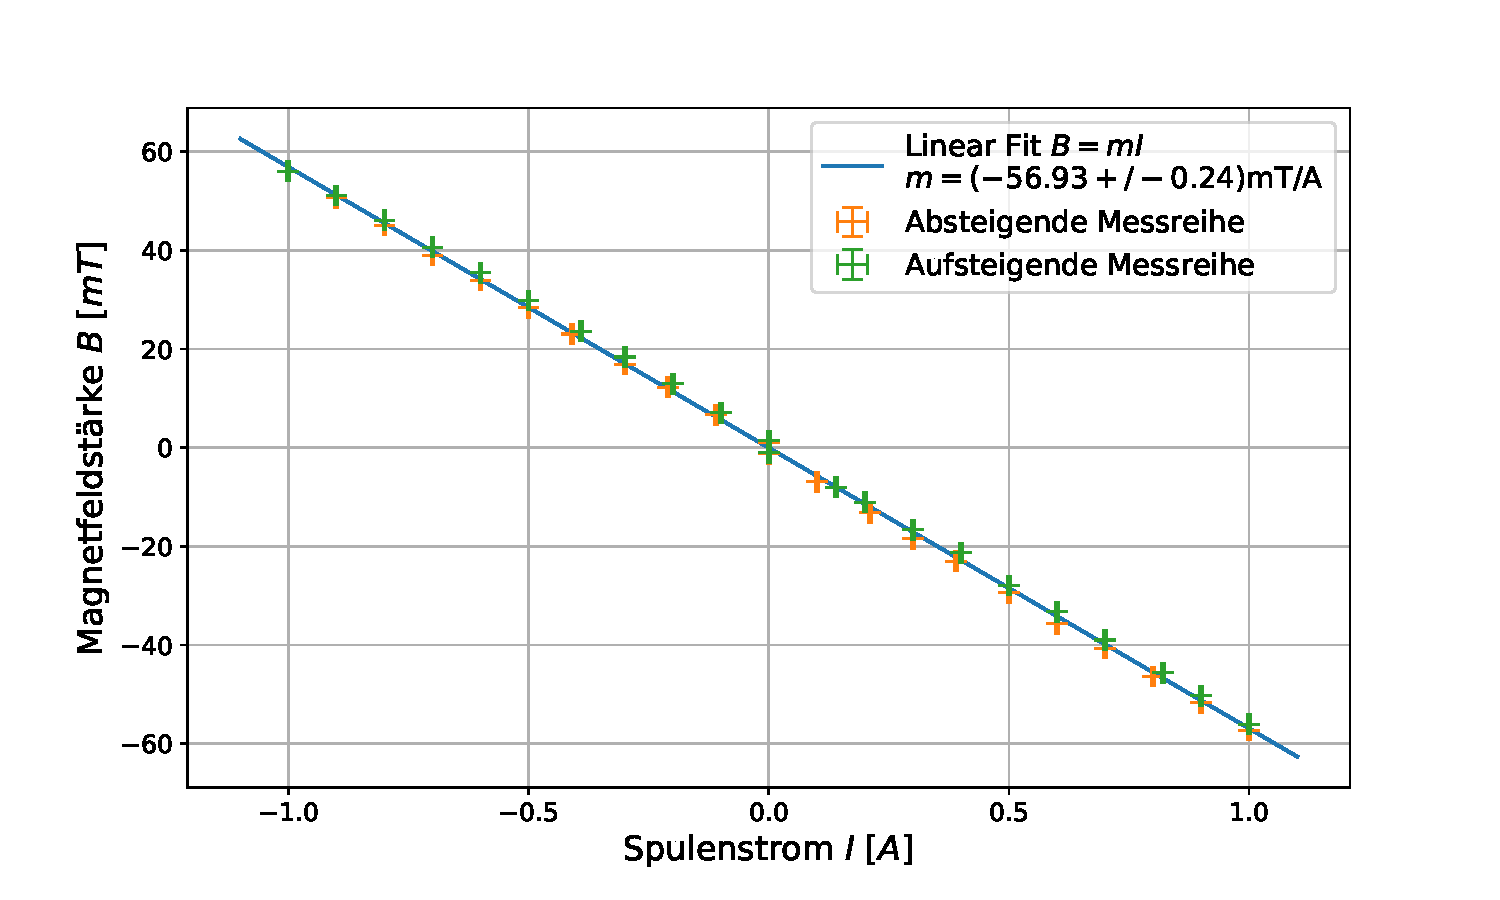
\includegraphics[width=\textwidth]{data/Magnetfeld.pdf}
		\caption{Messung der Magnetfeldstärke $B$ in Abhängigkeit der Stromstärke $I$ sowie linearer Fit.}
		\label{fig:Magnetfeld}	
	\end{figure}		
	Eine graphische Darstellung der aufgenommenen Messwerte für den ersten Teilversuch ist Abb. \ref{fig:Magnetfeld} zu entnehmen.
	Dabei sind die grünen Messpunkte die, welche von \SIrange{-1}{1}{\ampere} aufgenommen wurden und umgekehrt die orangefarbenen von \SIrange{1}{-1}{\ampere}.
	Aufgrund der Proportionalität zwischen $B$ und $I$, welche sich aus den Maxwell-Gleichungen ergibt, wurde ein linearer Fit gewählt.
	Alle Messpunkte liegen innerhalb einer Unsicherheit auf diesem Fit, welcher durch $B = m\cdot I$ mit $m = \SI{-56.93+-0.24}{\milli\tesla\per\ampere}$ beschrieben wird.
	
	\begin{figure}[ht]
		\centering
		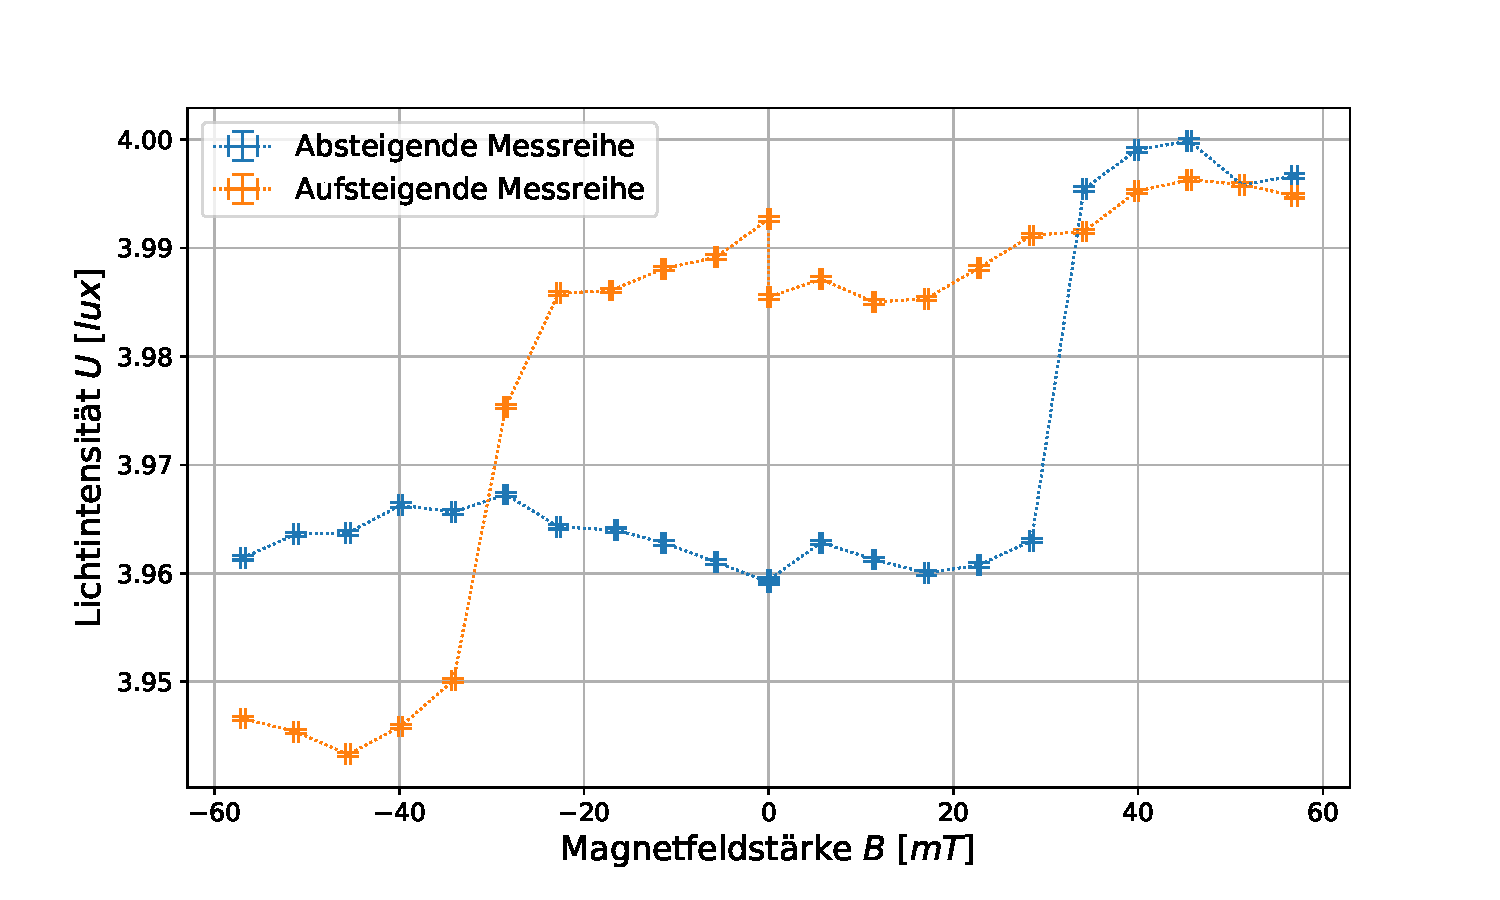
\includegraphics[width=\textwidth]{data/Hysterese.pdf}
		\caption{Messung der Lichtintensität $U$ in Abhängigkeit der Magnetfeldstärke $I$. Die gestrichelten Linien dienen nur zur Veranschaulichung und entsprechen nicht dem exakten Verlauf.}
		\label{fig:Hysterese}	
	\end{figure}
	Die Messkurve für den zweiten Teilversuch ist in Abb. \ref{fig:Hysterese} dargestellt. 
	Zu beachten ist, dass die gestrichelten Linien nur zur Veranschaulichung des Verlaufs dienen und in der Auswertung keine Rolle spielen.
	Wie bei der ersten Messung sind die Messpunkte farblich getrennt.
	Dabei sind die orangefarbenen Messpunkte die von \SIrange{56.93+-0.24}{-56.93+-0.24}{\milli\tesla} für die Magnetfeldstärke $B$ laufen und die blauen wiederum von \SIrange{-56.93+-0.24}{56.93+-0.24}{\milli\tesla}.
	Auffällig ist, dass bei ca. $\SI{-30}{\milli\tesla}$ für die eine und bei ca. $\SI{30}{\milli\tesla}$ für die andere Messreihe ein deutlicher Sprung in der Lichtintensität stattfindet.
	Zudem liegen die Endpunkte sehr dicht aneinander, für die Startpunkte gilt dies nicht.
	Unabhängig von den genauen Messwerten ließ sich jedoch ein nahe zu punktsymmetrischer Verlauf der beiden Messkurven erkennen. 
			
\section{Diskussion}
			
	Ziel des Versuches ist es eine Übereinstimmung zwischen den Beobachtungen und der Theorie hinter dem magneto-optischen Kerr-Effekt zu finden.
	Es stellt sich also die Frage, wie die Messergebnisse mit dieser Theorie korrelieren.
	Dazu zunächst zu der Bestimmung der magnetischen Feldstärke $B$ als Funktion der Stromstärke $I$:
	Wie bereits in Abschnitt \ref{sec:Analyse} angemerkt, folgt aus den Maxwell-Gleichungen, dass $B\sim I$ gilt.
	Dies stimmt mit der Messung überein, da jeder Messpunkt auf dem linearen Fit innerhalb einer Unsicherheit auffinden ließ.
	Für die Funktion ergab sich: $B = \SI{-56.93+-0.24}{\milli\tesla\per\ampere}\cdot I$.
	Mit diesem Verhältnis ließ sich die Messung der Lichtintensität in Abhängigkeit der magnetischen Feldstärke $B$ statt der Stromstärke $I$ ausdrücken.
	Dass die Lichtintensität hinter dem zweiten Polarisator bzw. dem Analysator sich ändert deutet auf eine Änderung der Polarisation hin.
	Der Grund für diese ist die Co/Pt-Probe bzw. das Magnetfeld dieser.
	Bei der Probe handelt es sich nämlich um einen Ferromagneten, also einem Material, welches auch ohne äußeres Feld eine Magnetisierung $M$ aufweist.
	Diese Magnetisierung lässt sich durch das Anlegen eines äußeren Magnetfeldes ändern.
	Eine Änderung der Magnetisierung führt zu einer Änderung Lichtintensität.
	Die beiden Größe sind also proportional zueinander und die Magnetisierung lässt sich somit durch die Messung der Lichtintensität in Abhängigkeit der Magnetfeldstärke $B$ darstellen.
	Nun zurück zu der Polarisationsänderung an der Co/Pt-Probe.
	Hierbei wird das zunächst linear (senkrecht) polarisierte Licht des Lasers elliptisch polarisiert.
	Dies geschieht dadurch, dass nach dem Kerr-Effekt links- und rechtspolarisiertes Licht in einem ferromagnetischem Material unterschiedlich gebrochen werden.
	Da linear polarisiertes Licht aus zwei gleichen, zueinander gegenläufigen, zirkulären Anteilen besteht, werden diese gleichen Anteile unterschiedlich gebrochen und das reflektierte Licht ist daraufhin elliptisch polarisiert.
	Die elliptische Polarisation lässt sich auch über den Kerrwinkel $\Theta_K$ und die Kerr-Elliptizität $\epsilon_K$ beschreiben, worauf an dieser Stelle jedoch verzichtet wird.
	
	Abbildung \ref{fig:Hysterese} stellt die Lichtintensität $U$ in Abhängigkeit der magnetischen Feldstärke $B$ dar.
	Dieser Verlauf ist also proportional zu dem der Magnetisierung $M$ in Abhängigkeit der magnetischen Feldstärke $B$.
	% Sei $\kappa$ der Proportionalitätsfaktor in $[\si{\ampere\per\meter\per\lux}]$.
	An den Enden des Graphs finden kaum noch Änderungen an, bei $B = \pm\SI{56.93+-0.24}{\milli\tesla\per\ampere}$ wird bereits die Sättigungsmagnetisierung $M_S$ erreicht.
	Der Verlauf des Graphs sollte einer sogenannten Hysteresschleife gleichen und punktsymmetrisch sein.
	Bei der Sättigungsmagnetisierung an dem rechten Ende liegen die Messpunkte fast aufeinander, wie sie es bei einer Hystereseschleife sollten, an dem linken Ende ist dies jedoch nicht so.
	Dennoch wirken die Verläufe der beiden Messreihen im Wesentlichen punktsymmetrisch.
	Der Fehler bei diesem Verlauf lässt sich auf die Empfindlichkeit des Systems zurückführen.
	Es ist nicht unwahrscheinlich, dass aufgrund einer leichten Erschütterung eines der Versuchsmaterialien leicht versetzt hat oder dass es in dem Raum zur Aufnahme dieser Werte etwas heller/dunkler wurde und sich deswegen die Intensität an der Photodiode leicht änderte.
	Ein Hysteresenverlauf ist der Messkurve dennoch deutlich zu entnehmen.
	Der Grund für diesen Verlauf ist die Bewegung der sogenannten Domänenwände in dem Ferromagneten, welche nicht reibungsfrei stattfindet.
	Die Domänenwände teilen die Magnetisierung in dem Ferromagneten in ihre Richtungsanteile.
	Wird eine Domäne größer so nähert sich die Magnetisierung der Richtung der entsprechenden Domänenmagnetisierung zu.
	Auffällig für den Hystereseverlauf sind die Werte bei $B = 0$ und $B = B_C \approx \pm \SI{30}{\milli\tesla}$.
	Bei ersterem ist die remanente Magnetisierung $M_R$ zu erkennen und dass diese je nach Durchlaufrichtung gerade gespiegelt liegt.
	Hingegen bei $B_C$ wird die Koerzitivfeldstärke erreicht, welche benötigt wird um die Magnetisierung $M$ umzudrehen.
	An diesen beiden Stellen ist in dem Graphen ein nahezu senkrechter Anstieg/Abfall zu erkennen.
	Hier ändert sich die Magnetisierung also am stärksten.
	
	All diese Beobachtungen ließen sich in den höheren Kontext einordnen, der dem magneto-optischen Kerr-Effekt zu Grunde liegt.
	Das Ziel dieser Untersuchung wurde somit erreicht.
	